In this chapter we introduce a novel pixel-based readout concept for TPCs.
Pixel based readouts offer several advantages over the traditional wire readout \citep{lartpc_recon_problems_joshi_2015}.
A key improvement offered from pixelization is true 3-D image reconstruction.
This allows for sharper vertex reconstruction, thereby improving the overall resolution of DUNE and decreasing the required time for a NP measurement.

Other advantages are ease of data analysis and a reduction in total data storage.
A pixel based readout automatically records two of the three spatial dimensions, and thereby provides for simpler analysis.
Additionally, the pixelated readout method presented here cuts the total required data storage and data acquisition rate (without loss to precision) by several orders of magnitude.

However, the advantages also come with the cost of increased design complexity as the number of readout channels increases by more than three orders of magnitude. 
The traditional wire based readout within a DUNE module will include hundreds to thousands of channels, whereas a full DUNE module with a pixel-based readout will have 10's of millions of channels.
This number of required channels to be stably readout during DUNE's expected lifetime ($\approx 20$ years), where the electronics continually operate at liquid argon temperatures is likely the largest hurtle for a pixel-based design.
The aim of this dissertation is to address the channel-size problem.

\section{Q-Pix: The Circuit Level Design}

The fundamental readout circuit~(\ref{fig:qpixCircuit}) was first introduced by Nygren and Mei~\citep{qpix:nygren:mei}.
The principle of the front-end circuit operates on measuring the the time of the output of a trigger which is connected to an integrating capacitor circuit.
The key difference of this readout circuit is that the measured value is time, not voltage or charge.
Such a design choice then allows this readout to only provided data when there is charge.

The circuit input is connected to the anode of a TPC where drifted electron charge accumulates.
Voltage is then built up from the charge stored on the pixel based on the capacitance according to the equation:

% what to say about genetic multiplexing?
% This differs from other concepts such as Genetic Multiplexing (\citep{PROCUREUR2013888_genetic_multiplexing}) and using only regions of interest (ROI).

\begin{equation}
Q_{i} = C_{i}V_{i}
\end{equation}
~\label{eq:capacitor}

After the capacitor voltage ($V_{i}$) exceeds a set threshold value the schmitt trigger activates.
The time of the trigger output is recorded by a digital logic which encodes this data as a 32 bit value.
Since the capacitor reset happens at the same time as the issued trigger the digitally-recorded value is the reset time.

\begin{figure}[]
\centering
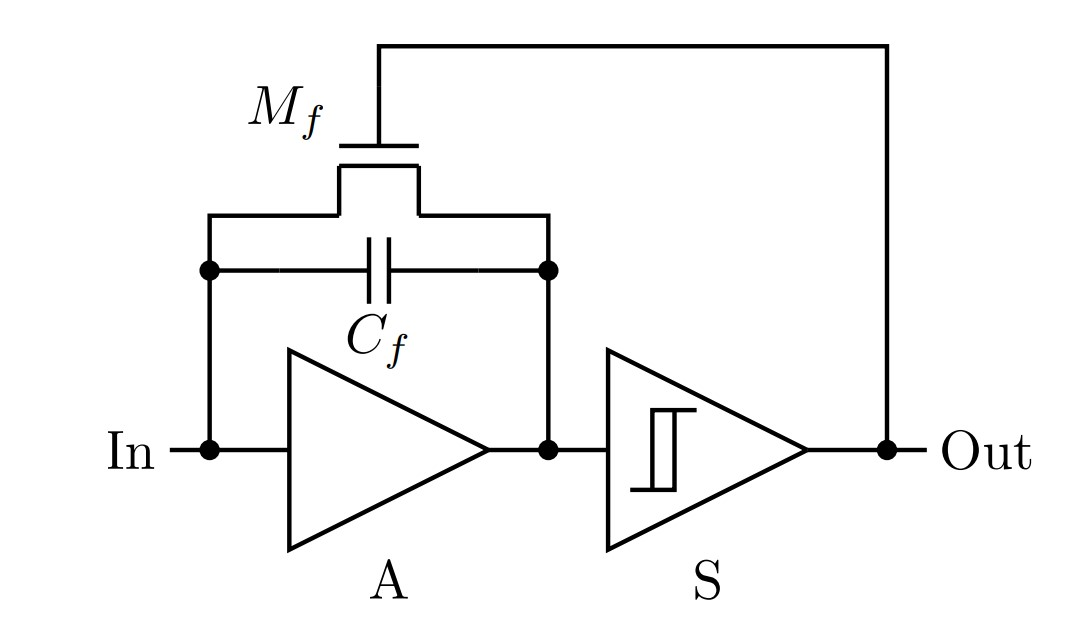
\includegraphics[width=\textwidth]{images/qpix_circuit.jpg}
\caption{Image of Basic Q-Pix Readout circuit. Currently this front-end circuit is being designed as custom analog ASIC which has 16 channels. Image is taken from \citep{qpix:nygren:mei}.}
\end{figure}
~\label{fig:qpixCircuit}

This timestamp value is recorded against a free running local oscillator ($f_{o} = 30\unit{MHz}$ ).
The number of free running clocks in the entire system is expected to be the number of channels ($N_{c}$) divided by the number of digitally multiplexed channels ($N_{d}$), which are taken to be 16.

\subsection{Waveforms from Time Resets}

Here we describe the basic principle of reconstructing the input current from a collection of reset measurements.
The key insight for this readout technology is that time (instead of voltage as in a MWPC) is recorded.
Therefore, measurements only taken place when there is enough charge to cause a reset which prevents continuous measurements during periods of long dead time.
This concept follows the detector concept of least action in that all measurements are detector responses.

A measurement of a reset indicates that a certain amount of charge was discharged from the integrating capacitor.
Since total charge is conserved (and assume drift current around the integrator is small compared to backgrounds), we can say that the total amount of charge that accumulates onto the pixel is equal to total amount of charge discharged from each reset, plus any residual charge still on the pixel.
Therefore, we can relate the total accumulated charge to the total charge discharged with the following equation:

\begin{equation}
Q_{in}(t) = Q_{out}(t) + Q_{c}(t)
\end{equation}
~\label(eq:qin)

If we assume that each reset removes the same amount of charge during each reset then we can rewrite the total charge out ($Q_{out}$) in terms of the integer number of resets at time t ($N(t)$):
\begin{equation}
Q_{out}(t) = Q_{o} N(t)
\end{equation}
~\label(eq:qout)

Where $Q_{o}$ is the fixed amount of charge discharged during each reset.
Equation~\ref{eq:qout} then can give us the measured current by definition ($I = \frac{dQ}{dt}$):
\begin{equation}
I_{o} = \frac{d}{dt}(Q_{o} \times N(t)) = Q_{o}\frac{dN}{dt} = \frac{Q_{o}f_{o}}{N_{clk}}
\end{equation}
~\label(eq:irecon)

Where we identify $\frac{dN}{dt} = \frac{f_{o}}{N_{clk}}$ as the as the clock frequency ($f_{o}$) of the local clock and the difference between the two resets.
Equation~\ref{eq:irecon} can be used to determine the maximum current with the digital clock frequency by noting that the minimal value of $N_{clk}$ is one.
We take as the nominal expected frequency (30~\unit{MHz}), capacitance (1~\unit{fF}), and voltage (1~\unit{V}) values to calculate an approximate max current, $I_{max}$:

\begin{equation}
I_{max} \approx 1~fF * 1~V * 30*10^{6} MHz \approx 30~nA
\end{equation}~\label{eq:icalc_max}

We note that 30 nA is much greater than the expected background current from $Ar^{39}$ ($\mathcal{O}(10^{-18})A$).
However, more interesting events deposit more more charge.
We can use the average drift speed of electrons in a LArTPC to estimate the maximum charge density such a configuration is sensitive to:

\begin{equation}
\lambda_{max} = \frac{dQ}{dL} = \frac{dQ}{dt} / \frac{dx}{dt} = \frac{I_{max}}{v_{drift}}
\end{equation}
~\label{eq:lambdaMax}

We use a nominal $v_{drift}$ speed of 1.6~\unit{mm} / $\mu$s, and convert to SI units to obtain $\lambda_{max}$ in equation~\ref{eq:lambdaMax}:
\begin{equation}
\lambda_{max} = \frac{3*10^{-8} A}{1600 \frac{m}{s}} = 1.875*10^{-11} \frac{C}{m} \approx 19 \frac{nC}{mm}
\end{equation}
~\label{eq:lambdaCalc}

We can now use this result to calculate a maximum $\frac{dE}{dx}$ measurement:

\begin{equation}
\frac{dE}{dx}_{max} = \frac{dQ}{dx}_{max}\frac{dE}{dQ} = \lambda_{max}\frac{dE}{dQ}
\end{equation}
~\label{eq:dedxMax}

We can take the ionization energy of $Ar^{39}$ to be $W_{ion} \approx 23.6 eV$, then:
$$
W_{ion} = \frac{23.6 eV}{e^{-}}
$$
and
$$
Q = 1.602*10^{-19} C
$$

Then $\frac{dE}{dQ}$ becomes:
\begin{equation}
\frac{dE}{dQ} = \frac{23.6 eV}{1.602\times 10^{-19} C}
\end{equation}
~\label{eq:dedxValue}

Finally, we calculate the result of equation~\ref{} and convert to units of~$\frac{GeV}{mm}$.
\begin{equation}
\frac{dE}{dx}_{max} = 1.875\times 10^{-11} \frac{C}{m} \times  \frac{23.6 eV}{1.602\times 10^{-19} C} \approx 2.76 \frac{MeV}{mm}
\end{equation}
~\label{eq:dedxCalc}

Next we aim to provide an estimate on the lower limit of detection for an event.
What follows provides a rough estimate for a potential lower bound on signal identification in the analysis, and note that a more thorough investigation of a true lower limit would require more work and beyond the scope of the work presented here.

First, we take as a lower bound estimate that any signal detection for an event purely based on charge reconstruction must provide more resets than background due to $Ar^{39}$ beta-decay.
Since the background rate from the dominate source is expected to provide resets of frequency $\approx 1\unit{Hz}$, an order of magnitude estimate for the minimal detectable current can be measured if we assume a signal-to-noise ratio (S/N) of 10.
Then, a detectable signal rate should deposit enough charge to trigger a reset within a time window of $\approx 0.1 \unit{s}$.

Following equation~\ref{eq:ical};
\begin{equation}
I_{min} \approx \frac{1~fF \times  1~V}{0.1 \unit{s}} \approx 10~\unit{fA}
\end{equation}~\label{eq:icalc_min}

We use $I_{min}$ to calculate an average charge line-density above the pixel, and again assume a constant drift speed, $v_{e} \approx 0.1601 \unit{cm/\mu s}$, from table~\ref{tab:lar_prop}.

\begin{equation}
\lambda_{min} = \frac{10^{-14} A}{1600 \frac{m}{s}} = 6.25\times 10^{-18} \frac{C}{m} \approx 6.25 \frac{aC}{m}
\end{equation}
~\label{eq:lambdaMin}

Finally, we calculate the minimum $\frac{dE}{dX}$ following~\ref{eq:dedxCalc}:
\begin{equation}
\frac{dE}{dx}_{min} = 6.25\times 10^{-18} \frac{C}{m} \times  \frac{23.6 eV}{1.602\times 10^{-19} C} \approx 0.921 \frac{eV}{mm}
\end{equation}
~\label{eq:dedxMin}

\begin{figure}[]
\centering
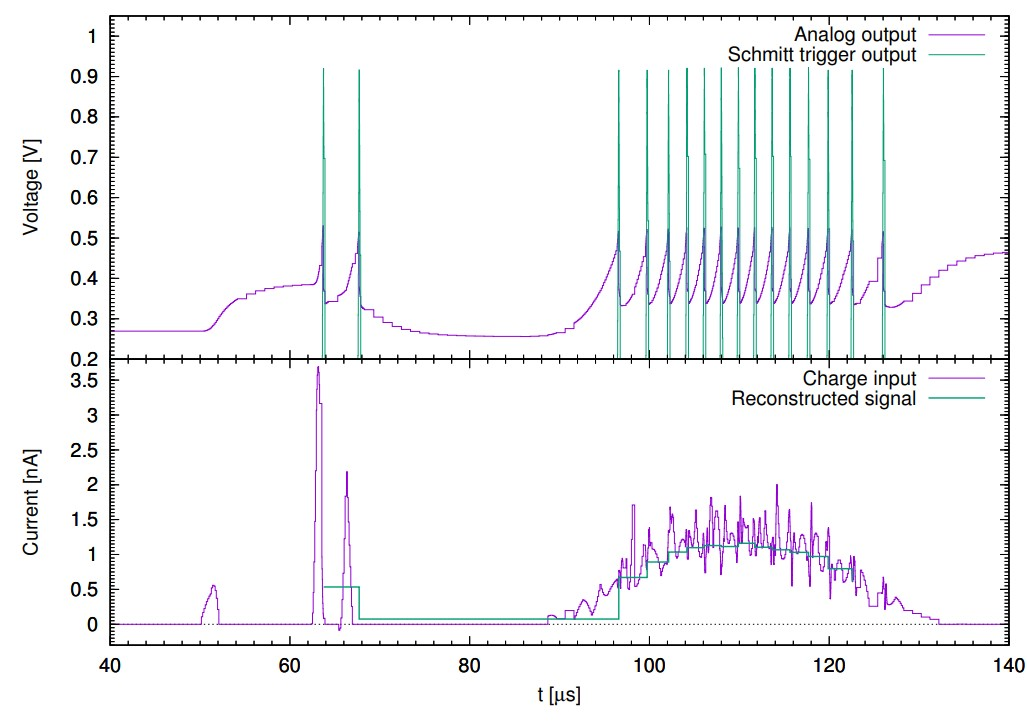
\includegraphics[width=\textwidth]{images/qpix_rtd_reconstruction_example.jpg}
\caption{Example reconstruction of the reset time difference (RTD) based on the Q-Pix readout design. Image is taken from \citep{qpix:nygren:mei}.}
\end{figure}
~\label{fig:qpixRecon1}

\begin{figure}[]
\centering
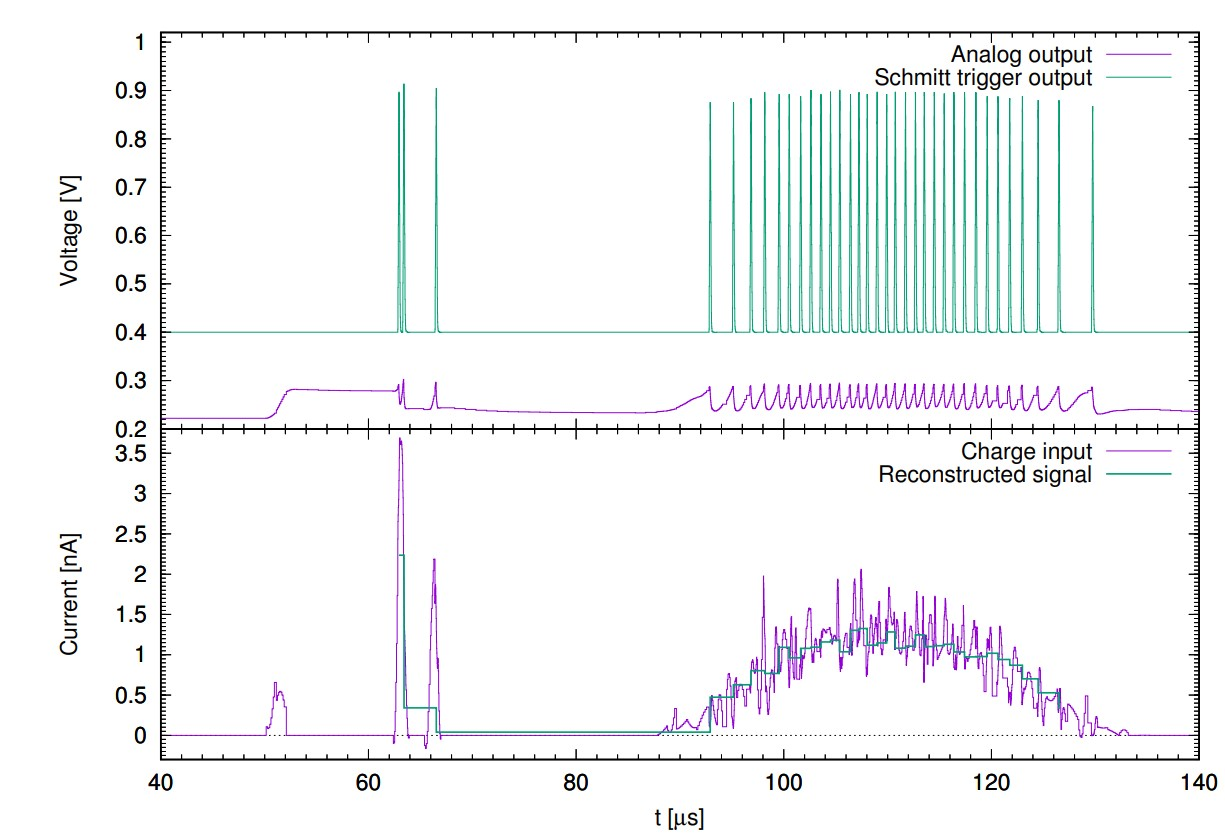
\includegraphics[width=\textwidth]{images/qpix_rtd_reconstruction_example_03fc.jpg}
\caption{Example reconstruction of the reset time difference (RTD) based on the Q-Pix readout design. delta-Q was chosen to be $0.3 fC$. Image is taken from \citep{qpix:nygren:mei}.}
\end{figure}
~\label{fig:qpixRecon2}

\subsection{Pixel Calibration}
~\label{sec:qpix_calib}

Calibration measurements are essential for any detector, as they provide a means to differentiate signal from noise.
Here we briefly describe an automatic use of existing $Ar^{39}$ decays as a source of calibration at the pixel level.
A full discussion of simulations using backgrounds is found in~\ref{chap:sim}.

The target volume (LAr) is stable nobel but still provides a quiescent background from the charge deposited $\beta$ decay ($\approx 6\unit{MeV}$).
The total volume continually observed by any pixel a drift distance $\approx$ 3.5\unit{m} yields an average reset on the order of 10s of seconds $\mathcal{O}(10^{1})$.
This value is much lower than the wrap-around rate of the 32-bit sample clock, which in practice will provide continually increasing reset values and prevent errors in identifying the correct reset time.

The pixel leevl value which needs to be calibrated is the pixel's response to an input charge $Q_{in}$ in equation~\ref{eq:capacitor}.
The capacitance ($C_{i}$) for each pixel is a systematic which can be calibrated periodically using the background current from $Ar^{39}$ decay.
Given some stable input charge, there is a known number of reset measurements to calibrate against.

LAr purity over the detector volume is essential for background calibration.
Differents in purity, electric, and maagnetic fields affect the major contributions to charge loss in the LAr: recombination, lifetime, and diffusion.

\subsection{Making a 3-D Image}

One of the important features of a TPC is the ability to reconstruct full 3-D images.
The intended benefit of a pixelated readout on any TPC is to show that there are improvements to reconstruction of these 3-D images.

In order to reconstruct the image of the interaction from a set of data above the pixel the required data are the reset time at a pixel i ($T_{ri}$), event time ($T_{e}$), and the pixel ID.
We assume that $T_{e}$ (as is normally used to tag events in TPCs) uses a trigger time from a secondary PMT system from the scintillation light produced by the interaction to tag an event of interest.
Since the scintillation photons travel much faster than the drift electrons, we can use the $T_{e}$ as the starting time.

The pixel ID of each reset gives two of the three remaining coordinates ($\hat{x}$ and $\hat{y}$).
The last coordinate ($\hat{z}$) is reconstructed using $T_{ri}$.

% average value is 1.6 mm / us from Nygren's QPix paper.
Since the drift velocity of the electrons ($v_{e}$) is constant in a TPC the distance that the electrons traveled to reach the anode plane ($\hat{z}$) is determined based on only the drift time:
\begin{equation}
  z = v_{e} * T_{drift}
\end{equation}~\label{eq:driftDistance}

However, this drift time is measured directly from the difference between the event time ($T_{e}$) and the reset time for this pixel ($T_{ri}$).
\begin{equation}
  T_{drift} = T_{ri} - T_{e}
\end{equation}

The drift distance in equation~(\ref{eq:driftDistance}) becomes:
\begin{equation}
  z = v_{e} * (T_{ri} - T_{e})
\end{equation}~\label{eq:driftDistanceCalc}

\subsection{Bad Scenarios}

Here we briefly describe potential issues of the readout circuit presented here.

\subsubsection{Near Maximum Reset Rate}

Equation ~\ref{eq:icalc_max} relates the maximum measurable current ($I_{max}$) in a QPix system to the frequency of a digital clock.

The general relationship for the curret is given in equation~\ref{eq:icalc_max}.
This can be rewritten explicitly in terms of the number of measured clock counts at the remote ASIC:
\begin{equation}
  I_{r}(N_{clk}) = \frac{Q_{o}f_{o}}{N_{clk}}
\end{equation}~\label{eq:i_clk}

Where $f_{o}$ is the nominal frequency of the free running remote clock, and $N_{clk}$ is the 32-bit encoded timestamp.

We note here that because $N_{clk}$ can only take positive integer values that there can be large uncertainty in the measured currents between the maximum and half of the maximum.
That is since $I(t) \simeq 1/N_{clk}$, explicitly measured currents can only be discrete and have large variance for small $N_{clk}$.

However, these discrete uncertainties can be accounted for after digital processing.
An example of a periodic artificial input current of with $I \approx I_{max}/10$ is shown below in Figure~\ref{fig:savgol}.
The reconstructed charge over time is shown in Figure~\ref{fig:reconQ}.

\begin{figure}[]
\centering
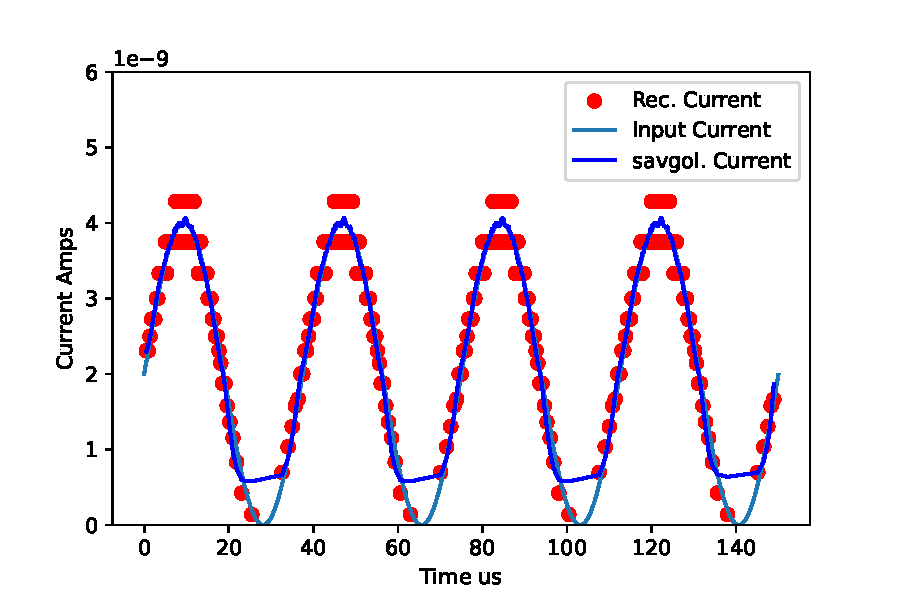
\includegraphics[width=\textwidth]{images/savgol.pdf}
\caption{Arbitrary sin-wave based current input. Maximum amplitude is chosen to be close to $I_{max}$. Reset Charge is chosen to be 1 $\unit{fC}$ and digital clock frequency of 30 $\unit{MHz}$. Since the amplitude is close to the maximum, and the clock measuremets are necessarily discrete, the exact current can not be measured from reset-to-reset. However, an example of a savgol filter is performed on the resets after the fact, shown in blue, with near agreement of the large input. An use-case of this kind of digital filtering would be applied to large current values only, and not for low current inputs, where the pure timestamp difference provides better results.}
\end{figure}~\label{fig:savgol}

\begin{figure}
\centering
\begin{subfigure}{.5\textwidth}
  \centering
  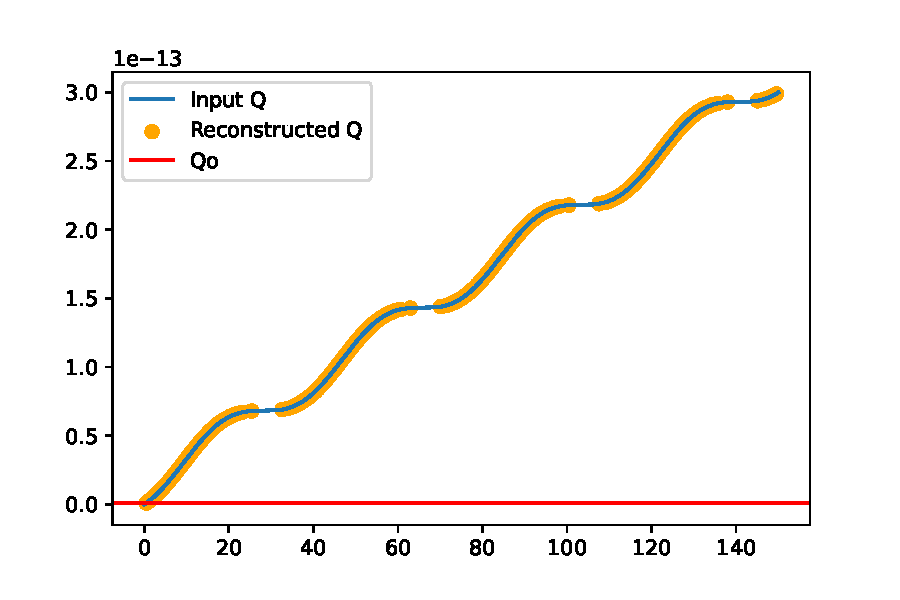
\includegraphics[width=\textwidth]{images/reconQ.pdf}
  \caption{CDF}
\end{subfigure}%
\begin{subfigure}{.5\textwidth}
  \centering
  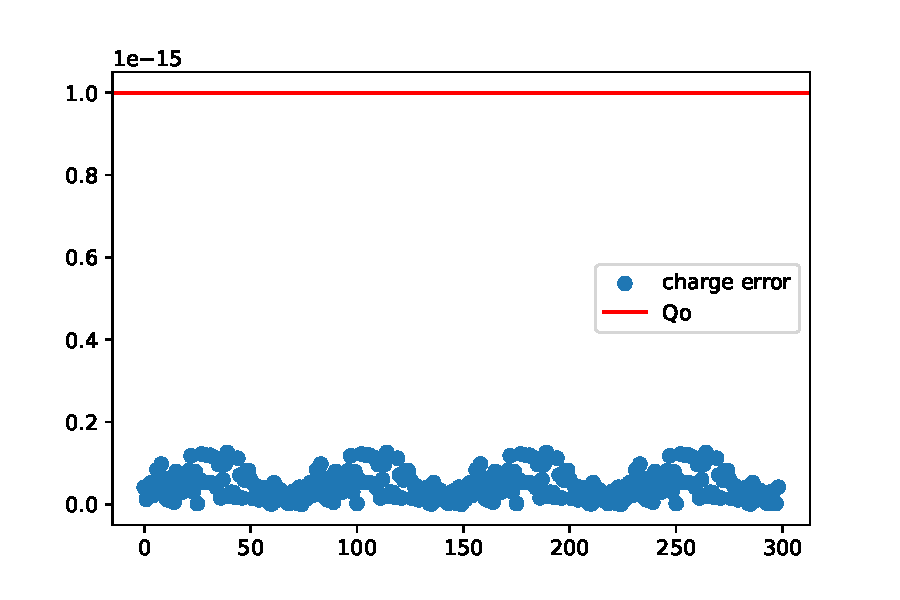
\includegraphics[width=\textwidth]{images/diffQ.pdf}
  \caption{Difference}
\end{subfigure}
\caption{Reconstruction of Sub figures CDF of charge as a function of time (a) and difference (b).}
\label{fig:reconQ}
\end{figure}

\subsubsection{Discussion of Uncertainties}

The uncertainty for the two transverse coordinates ($\hat{x}$ and $\hat{y}$) come from the pixel size.
If we assume the electric field to be uniform, on average, across all $\mathcal{O}(10^{7})$ pixels in an APA, then the charge drift will be uniformly distributed over the pixel size.
Then, the pixel dimensions determine the resolution: $\frac{3 mm}{\sqrt{12}} \approx 0.87 mm$.

The two remaining coordinates to reconstruct tracking are drift distance, $\hat{z}$, and then time the charge was deposited, $T_{ei}$.
The measurement of $\hat{z}$ is based on equation~\ref{eq:driftDistanceCalc}.
Expanding the uncertainties based on this equation, and assuming $v_{e}$ to be a constant, gives us a relation for $\sigma_{\hat{z}}$ to be:
\begin{equation}
  \sigma_{\hat{z}} = v_{e}(\sigma_{T_{ei}} +  \sigma_{T_{e}})
\end{equation}

Where $\sigma_{T_{ei}}$ and $\sigma_{T_{e}}$ are the uncertainties for the reconstructed charge arrival time and the event time, respectively.
Of these two, only $\sigma_{T_{ei}}$ depends on the reconstructed charge value; $T_{e}$ can be provided as an external trigger, such as a photonics system which uses scintillation photons.
Such a system can reasonably expected to have a much smaller uncertainty than $\sigma_{T_{ei}}$ since its timescale (ns) is three orders of magnitude smaller.

Therefore, to reasonable approximation $\sigma_{\hat{z}}$ is:
\begin{equation}
  \sigma_{\hat{z}} \approx v_{e}\sigma_{T_{ei}}
\end{equation}~\label{eq:zdrift_uncert}

Equation~\ref{eq:zdrift_uncert} relates the uncertainties of the last two coordinates which define a total event reconstruction.
A full treatment of the uncertainty in time ($\sigma_{T_{ei}}$) depends on the uncertainty of the measurement of the timestamps for each remote ASIC in a tile, as well as the charge per reset ($Q_{o}$) and nominal frequency of the ASIC ($f_{o}$).
The full treatment to analyze the uncertainty of $f_{o}$ is the goal of this work and the details are provided in Chapter~\ref{chap:qdb}.
The measurement of the uncertainty provided by the charge ($Q_{o}$) depends strictly on the analog front-end, which is beyond the scope of the work presented here.

We can provide here, however, an order of magnitude estimation based on equation~\ref{eq:eq:i_clk}, if we consider only the contribution of the uncertainty due to the measurement of time which depends on the number of clocks recorded since the last reset ($N_{clk}$).
Since the measurement of the input current is inversely proportional to $N_{clk}$, the percent uncertainty of the current measurement is proportional to the percent uncertainty in the timestamp measurement.

A 1\% measurement of error can be calculated using a standard percent error definition, and by noting that the maximmal error happens when a true current should record a value between $N_{clk}+1$ and $N_{clk}$ counts.
A maximal error of a measured current would happen if the current provides just shy the amount of charge to trigger a reset in $N_{clk}$ cycles and instead the recorded reset occurs on the next clock, $N_{clk} + 1$.
The worst case true measurement should be:
\begin{equation}
  N_{true} = \frac{1}{N_{clk}}
\end{equation}~\label{eq:ntrue}

We can then directly apply percent error:
\begin{equation}
  error = \frac{\frac{1}{N_{true}} - \frac{1}{N_{clk}+1}}{N_{true}}
\end{equation}

Plugging in the value $N_{true}$ from equation~\ref{eq:ntrue} and simplifying gives:
\begin{equation}
  error = \frac{1}{N_{clk}+1}
\end{equation}~\label{eq:nerr}

Equation~\ref{eq:nerr} provides a general formula for calculating the maximal error due to the discretization of the timestamp measurement.
Then, we can solve for $N_{clk}$ to determine how many clock cycles must occur between two resets for a 1\% error (error $= \frac{1}{100}$):
\begin{equation}
  N_{clk} \approx 100
\end{equation}

Then after 100 clock cycles, the worst possible measurement of the current is still within 1\%.
100 clocks cycles for a 30 $\unit{MHz}$ clock yields measured drift time $t_{drift} \approx$ 3.33 $\unit{\mu s}$.
The drift, $v_{e^{-}}$ is $\approx$ 1.6 $\unit{\frac{mm}{\mu s}}$, multiplied by the time gives the drift distance, known to within 1\%:
\begin{equation}
  \hat{z} = v_{e^{-}}t_{drift} \approx 3.33 \cdot 1.6 = 5.33 \unit{mm} \pm 0.05 \unit{mm}
\end{equation}~\label{eq:zdriftnclk}

We can rewrite equation~\ref{eq:zdriftnclk} explicitly in terms of $N_{clk}$ to get a worst case:
\begin{equation}
  \hat{z} = v_{e^{-}}\frac{N_{clk}}{f_{o}}
\end{equation}~\label{eq:zdriftworse}

The maximal percent error in the drift distance due to timing increases as $N_{clk}$ decreases, however because the drift distance is also calcuated using.

\section{How Q-Pix fits into a DUNE APA}~\label{sec:qpix_apa}

Here we briefly describe QPix system requirements at DUNE module size (10 kt).
A full technical design report for a kt module implementing QPix is clearly beyond the scope of the work presented here, yet we still offer comments on the requirements, particularly on the digital back-end related to a DUNE APA.

%% section 1.8 of TDR
DUNE's Anode Plane Assemblies (APA) full description can be found at~\citep{DUNE-FD_TDRv4:Abi_2020}.
Expected noise level of 1000 $e^{-}$.
Sampling frequency of 12 bit ADCs is 12 $\unit{MHz}$.
Expect to collect 20-30 $k e^{-}$ per channel for a minimum ionizing particle.
Large signals require a linear reponse of 500 k$e^{-}$, and ensures that fewer than 10\% of beam events experience saturation.

Dune APA takes 20 Front-End-Motherboards (FEMBs), to digitize a total of 128 wires.
40 wires are taken from the U and V (induction) layers, and 48 wires are taken from the X (conduction) layer.
The reason for this distribution is simply that that the X layer has a total of 980 wires per APA, where the U/V layers have 800 wires.

Three ASICs are responsible for collecting the charge as it passes between the wires and sending it out of the cryostat.
The first ASIC is a waveform-shaping and amplification ASIC.
The second ASIC is the ADC ASIC and is reponsible for converting the analoge signal to digital.
The final ASIC, called the COLDATA ASIC, merges the data streams from the previous ASICs and is responsible for communication between the motherboard and the outside world.
Maximum expected data collection is to exceed no more than 30 PB/year, which corresponds roughly to $\approx 1 Gb/s$ of continuous collection.

Each 10 kT module consists of 150 APAs.
Dune expects to draw less than 50 mW per channel, and less than 1\% dead channels.

Each APA is 6.324 $\unit{m}$ $\times$ 2.316 $\unit{m}$, for a total area of 14.646 $\unit{m^{2}}$.
Therefore, the expected channel count of a QPix APA is
\begin{equation}
  N_{pix} = 14.646 m^{2} * \frac{1 pixel}{4 mm^{2}} * \frac{ 1000^{2} mm^{2} }{m^{2}} = 915399
\end{equation}

To have a comparable power draw compared to DUNE, which has 2560 channels, then QPix would need less than $\approx 140 \mu W$ of power draw per channel.
Too much energy disappated in the LAr creates bubbles which is a high voltage (HV) discharge risk.
The total channel count for a 10 kT module is based on 150 DUNE-APAs or $2560\times 150 = 384000$.

Thus, the number of extra analog channels that QPix is required to measure, compared to the typical wire readout, increases by a factor of $915399 / 2560 \approx 357$.
This is an increase of $\mathcal{O}(10^{3})A$ orders of magnitude.


QPix instead offes conversion from analog (charge) to digital (32 bit time) signals on the front-end ASIC.
These front-end ASICs would be arrayed in tiles, and the tiles themselves would spread out to cover the entire area of an APA.
Each tile would interface with a single FPGA chip would would concentrate the digital data for each tile; we refer to this FPGA as the DAQ-Node (DN).
Then, each DAQ-Node interfaces with at least a single concentrator FPGA that sends the digital data to the Warm-Interface-Cards (WIC) out of the cold electronics (CE).
The final concentrator FPGA we refer to as the Super-DAQ-node (SDN).

The exact description and characteriziation of the WIC for a QPix depends on the final implementation of the SDN and is thus beyond the scope of the presented here.

\begin{figure}[]
\centering
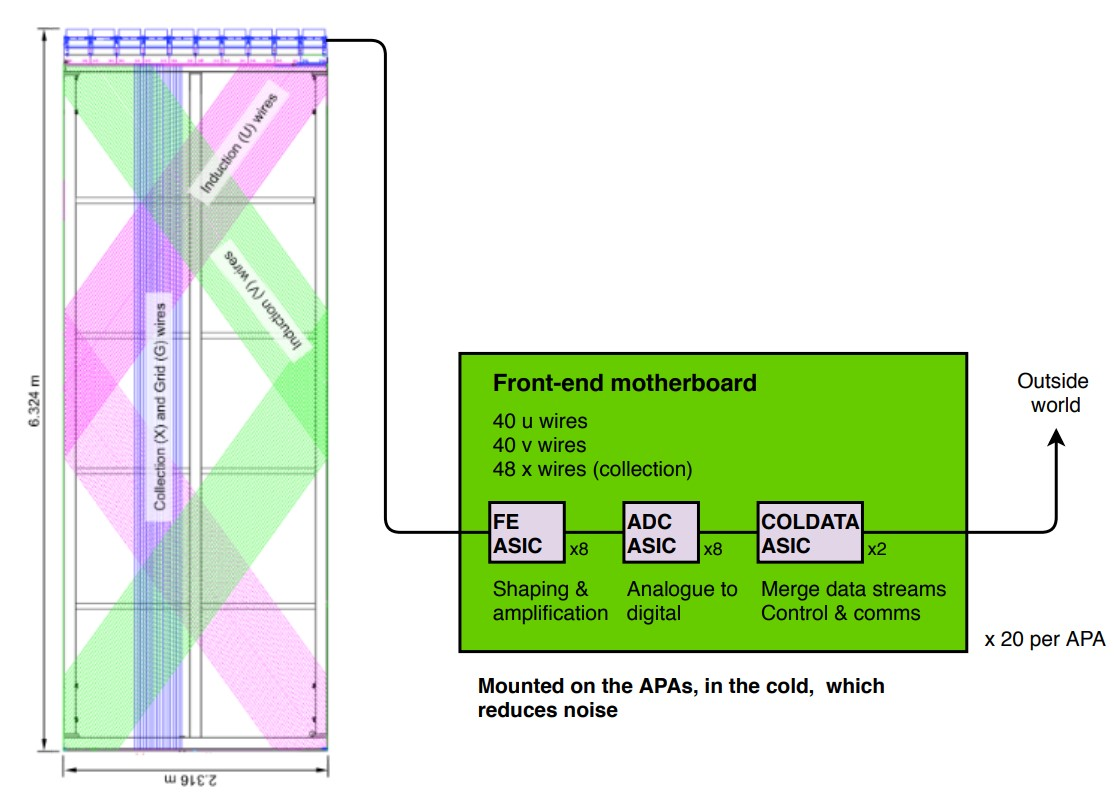
\includegraphics[width=\textwidth]{images/dune_apa_motherboards.jpg}
\caption{Image taken from~\citep{DUNE-FD_TDRv4:Abi_2020}, Fig 1.12 of section 1.8. Image shows an overlay the the relevant charge collection wires within a SP DUNE LArTPC.}
\end{figure}~\label{fig:dune_tpc_electronics}


%% example image of DUNE-APA from DUNE-FD TDR.
\begin{figure}[]
\centering
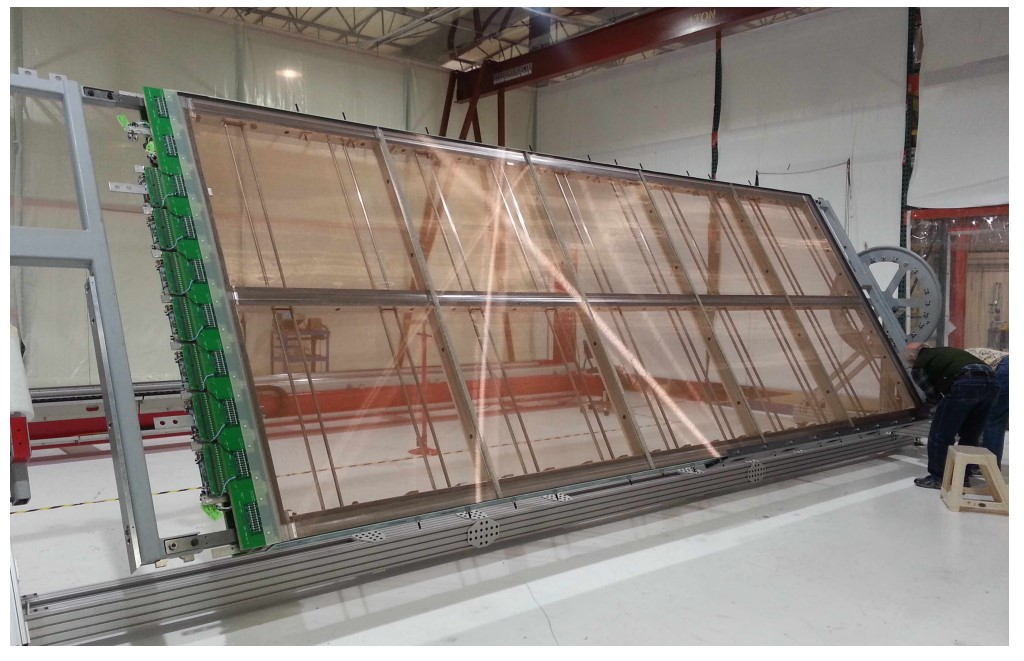
\includegraphics[width=\textwidth]{images/dune_fd_tdr_apa_image.jpg}
\caption{A simple caption \citep{DUNE-FD_TDRv4:Abi_2020}}
\end{figure}

\section{System Requirements}

We consider that the digital blocks responsible for digitizing the reset to have a nominal frequency of $\approx 30 MHz$.
Therefore, the minimum time before the recorded timestamp value resets is calculated by:

\begin{equation}
T_{loop} = \frac{2^{32}}{30\times 10^{6}} \approx 143 seconds
\end{equation}~\label{eq:tloop}

This time ($T_{loop}$) indicates the minimum reset time to occur within each responsible digital block.
Since this time is much greater than the antipcated reset rates to be produced from backgrounds, discussed in section~\ref{sec:qpix_calib}, we expect the looping of the 32-bit recorded value to not present a design concern.

The total number of free running oscillators ($N_{osc}$) per DUNE-APA for a given pixel pixel of $4~mm^{2}$ is:
\begin{equation}
N_{osc} = \frac{915399}{16} \approx 57213
\end{equation}~\label{eq:nosc}

$N_{osc}$ represents the total number of front-end ASICs whose data must be aggregated and sent outside of the cold electronics to a warm interface.
Therefore we expect the order of the number of free running oscillators per DUNE-APA $\mathcal{O}$($10^5$).
This also gives an order of magnitude estimate of the increase of number of ASICs compared to the MWPC readout of Single-Phase (SP) DUNE-FD.

Figure~\ref{fig:dune_tpc_electronics} shows that each APA uses 20 FEMBs to digitize 128 of the 2560 channels.
Each FEMB houses a total of 18 ASICs which smooth, digitize, and aggregate data before being sent to the Warm Interface CRATE (WIC).
The total number of ASICs per APA is $18\times 20 = 360$.
Since each 10 kt module uses 150 APAs the total number of ASICs would be multiplied by 150.

\begin{table}
\begin{center}
\begin{tabular}{|| p{50mm} | p{50mm} | p{50mm} ||}
 \hline
 Description & Specification & Rationale \\ [0.5ex]
 \hline\hline
  System Noise & < 1000 $e^{-}$ & Provides >5:1 S/N on induction planes for pattern recognition and two-track separation. \\
 \hline
  Signal Saturation & 500,000 $e^{-}$ & Maintain calorimetric performance for multi-proton final state. \\
 \hline
  Cold Electronics Power Consumption & < 50 mW pre channel & No bubbles in LAr to reduce HV discharge risk\\
 \hline
  Number of Channels per front-end motherboard & 128 &  The total number of wires on one side of an APA, 1,280, must be an integer multiple of the number of channels on the FEMBs. \\
 \hline
Maximum diameter of conduit enclosing the cold cables while they are routed through the APA frame. & 6.35 cm (2.5") & Avoid the need for further changes to the APA frame and for routing the cables along the cryostat walls \\
 \hline
\end{tabular}
\caption{Selected Requirements of DUNE TPC electronics and Expected QPix Design goals of first generation ASIC development for comparison. TPC electronic data and rationale are taken from~\citep{DUNE-FD_TDRv4:Abi_2020}}
\end{center}
\end{table}~\label{tab:dune_tpc_elec}

\begin{table}
\begin{center}
\begin{tabular}{|| p{50mm} | p{50mm} | p{50mm} ||}
 \hline
 Description & Specification & Rationale \\ [0.5ex]
 \hline\hline
  System Noise & $\approx 300 e^{-}$ & Provides $\approx$ 17:1 S/N ratio, a component of front-end integrator. \\
 \hline
  Signal Saturation & >30\unit{nA}? & Upper limit from local oscillator frequency and integrator reset. \\
 \hline
  Cold Electronics Power Consumption &  $< 100 \unit{\mu W}$ per channel & Equivalent power consumption for heating \\
 \hline
  Number of Channels per Tile & ?? &  Design parameter to be calculated. \\
 \hline
Maximum diameter of conduit enclosing the cold cables while they are routed through the APA frame. & 6.35 cm (2.5") & Same as~\citep{DUNE-FD_TDRv4:Abi_2020}, an engineering goal is to aim to use existing APA frame designs. \\
 \hline
\end{tabular}
\caption{Q-Pix based Requirements, which can be compared against~\ref{tab:dune_tpc_elec}. Results here are necessarily speculative, but provide a design goal baseline.}
\end{center}
\end{table}~\label{tab:qpix_tpc_elec}

The goal of a digital backend design is how to handle the data from the $10^{5}$ free running oscillators, and how to ensure that the free running local oscillator clocks can be calibrated to a known frequency.
Additionally,

\subsection{Single Point Failures}

Here we comment on an overall design guideline for Q-Pix: ``robust resilience'' against single point failure (SPF).
The readout technology presented here relies on huge numbers of readout channels ($10^{8}$) compared to current MWPC designs ($10^{5}$).
As such, extra care must be made in designing new technology to improve over established, seemingly simpler means.

This principal guides design choices such as the use of independent local oscillators at the pixel-level instead of a provided distributed clock.
This design choice, in particular, is discussed at length in chapter~\ref{chap:qdb}, and the findings presented there are one of the major contributions presented in this work.

The design which avoids SPF and handles the digital requirements presented here, namely: the continual time calibration of each local oscillator ($N_{osc} \approx 10^{5}$) is a goal of this work.

\section{Q-Pix and Light Detection}

Other recent progress~\citep{https://doi.org/10.48550/arxiv.2207.11127} has been made towards inclusion of an optical system combined the readout technology presented here.
Such a system would integrate well with a charge-integrate-reset style presented here, as the charge collection area is much smaller than the total pixel area.
The pixel dimensions are 4 $\unit{mm}$ $\times$ 4 $\unit{mm} $ for a total active area of 16$\unit{mm^{2}}$.
Most of this active area is unused for the charge collection pad, which could be as small as drill-hole via (6 mil $<<$ 16\unit{mm^2}).
Then, most of the remaining area could be plated with a photo-sensitive material.

Such a photosensitive material could capture incoming scintillation photons and provide an additional voltage measurement at each pixel.
Depending on the sensitivity, such a measurement could be used to reconstruct tracks by providing a $\frac{dE}{dX}$ measurement, or even as a time-tag and a trigger.

The use of a reference trigger could be useful to establish event-time within the same system, and allow adjacent pixels which would receive photons, but not charge, to contribute to time reconstruction.
Any reconstructed event requires some $T_{o}$ time to indicate the start of the event.
Typically this is done via scintillation photons from a secondary system, where the photons arrive nearly instantly at the collection planes compared to the slow drift speed of the electrons.

The natural pixelization of QPix required the charge collection can also be used to be sensitive to scintillation photons.
These photons could not only provide the required timing but also provide an additional means of calorimetry, and track reconstruction.
Additional work is currently underway to demonstrate the viability.
